\documentclass{article}
\usepackage{tikz}
\usetikzlibrary{graphs}
\usetikzlibrary{arrows.meta}

\pgfdeclarearrow{
  name=BigGlyph,
  cache=false,
  bending mode=none,
  drawing code={
    \pgfpathrectangle{\pgfpoint{-1.5ex}{-1ex}}{\pgfpoint{+2ex}{+2.5ex}}
    \pgfusepathqclip
    \pgftransformxshift{+0.1ex}
    \pgftransformyshift{-0.8ex}
    \pgftext[right,base]{$\mathsf{Z}$}
  }
}

\pgfdeclarearrow{
  name=SmallGlyph,
  cache=false,
  bending mode=none,
  parameters={},
  drawing code={
    \pgfpathrectangle{\pgfpoint{-1.5ex}{-1ex}}{\pgfpoint{+2ex}{+2.5ex}}
    \pgfusepathqclip
    \pgftransformxshift{+0.1ex}
    \pgftransformyshift{-0.5ex}
    \pgftext[right,base]{$\mathsf{p}$}
  }
}

\begin{document}
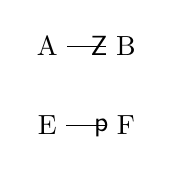
\begin{tikzpicture}
    \node (A){A};
    \node (B)[right of=A] {B};
    \node (E)[below of=A] {E};
    \node (F)[right of=E] {F};
    \draw [-{BigGlyph}] (A) to (B);
    \draw [-{SmallGlyph}] (E) to (F);
\end{tikzpicture}
\end{document}

